\section{Convolution of Exponential Functions}
	Let's choose $f(t) = e^{-at}$ for $a > 0$ as our input signal.
	
	The convolution is:
	\begin{equation}
		y(t) = \int_{-\infty}^{\infty} e^{-a\tau} \cdot h(t - \tau) d\tau
	\end{equation}
	
	Since $h(t - \tau)$ is non-zero only when $-T \leq t - \tau \leq T$, or $t - T \leq \tau \leq t + T$, the effective integration limits are:
	\begin{equation}
		y(t) = \int_{t-T}^{t+T} e^{-a\tau} d\tau
	\end{equation}
	
	Computing this integral:
	\begin{align}
		y(t) &= \int_{t-T}^{t+T} e^{-a\tau} d\tau \\
		&= \left[ -\frac{1}{a}e^{-a\tau} \right]_{t-T}^{t+T} \\
		&= \frac{e^{-at}}{a}(e^{aT} - e^{-aT})
	\end{align}
	
	Using the definition of hyperbolic sine, we can write:
	\begin{equation}
		y(t) = \frac{2\sinh(aT)}{a}e^{-at}
	\end{equation}
	
	\begin{figure}[htbp]
		\centering
		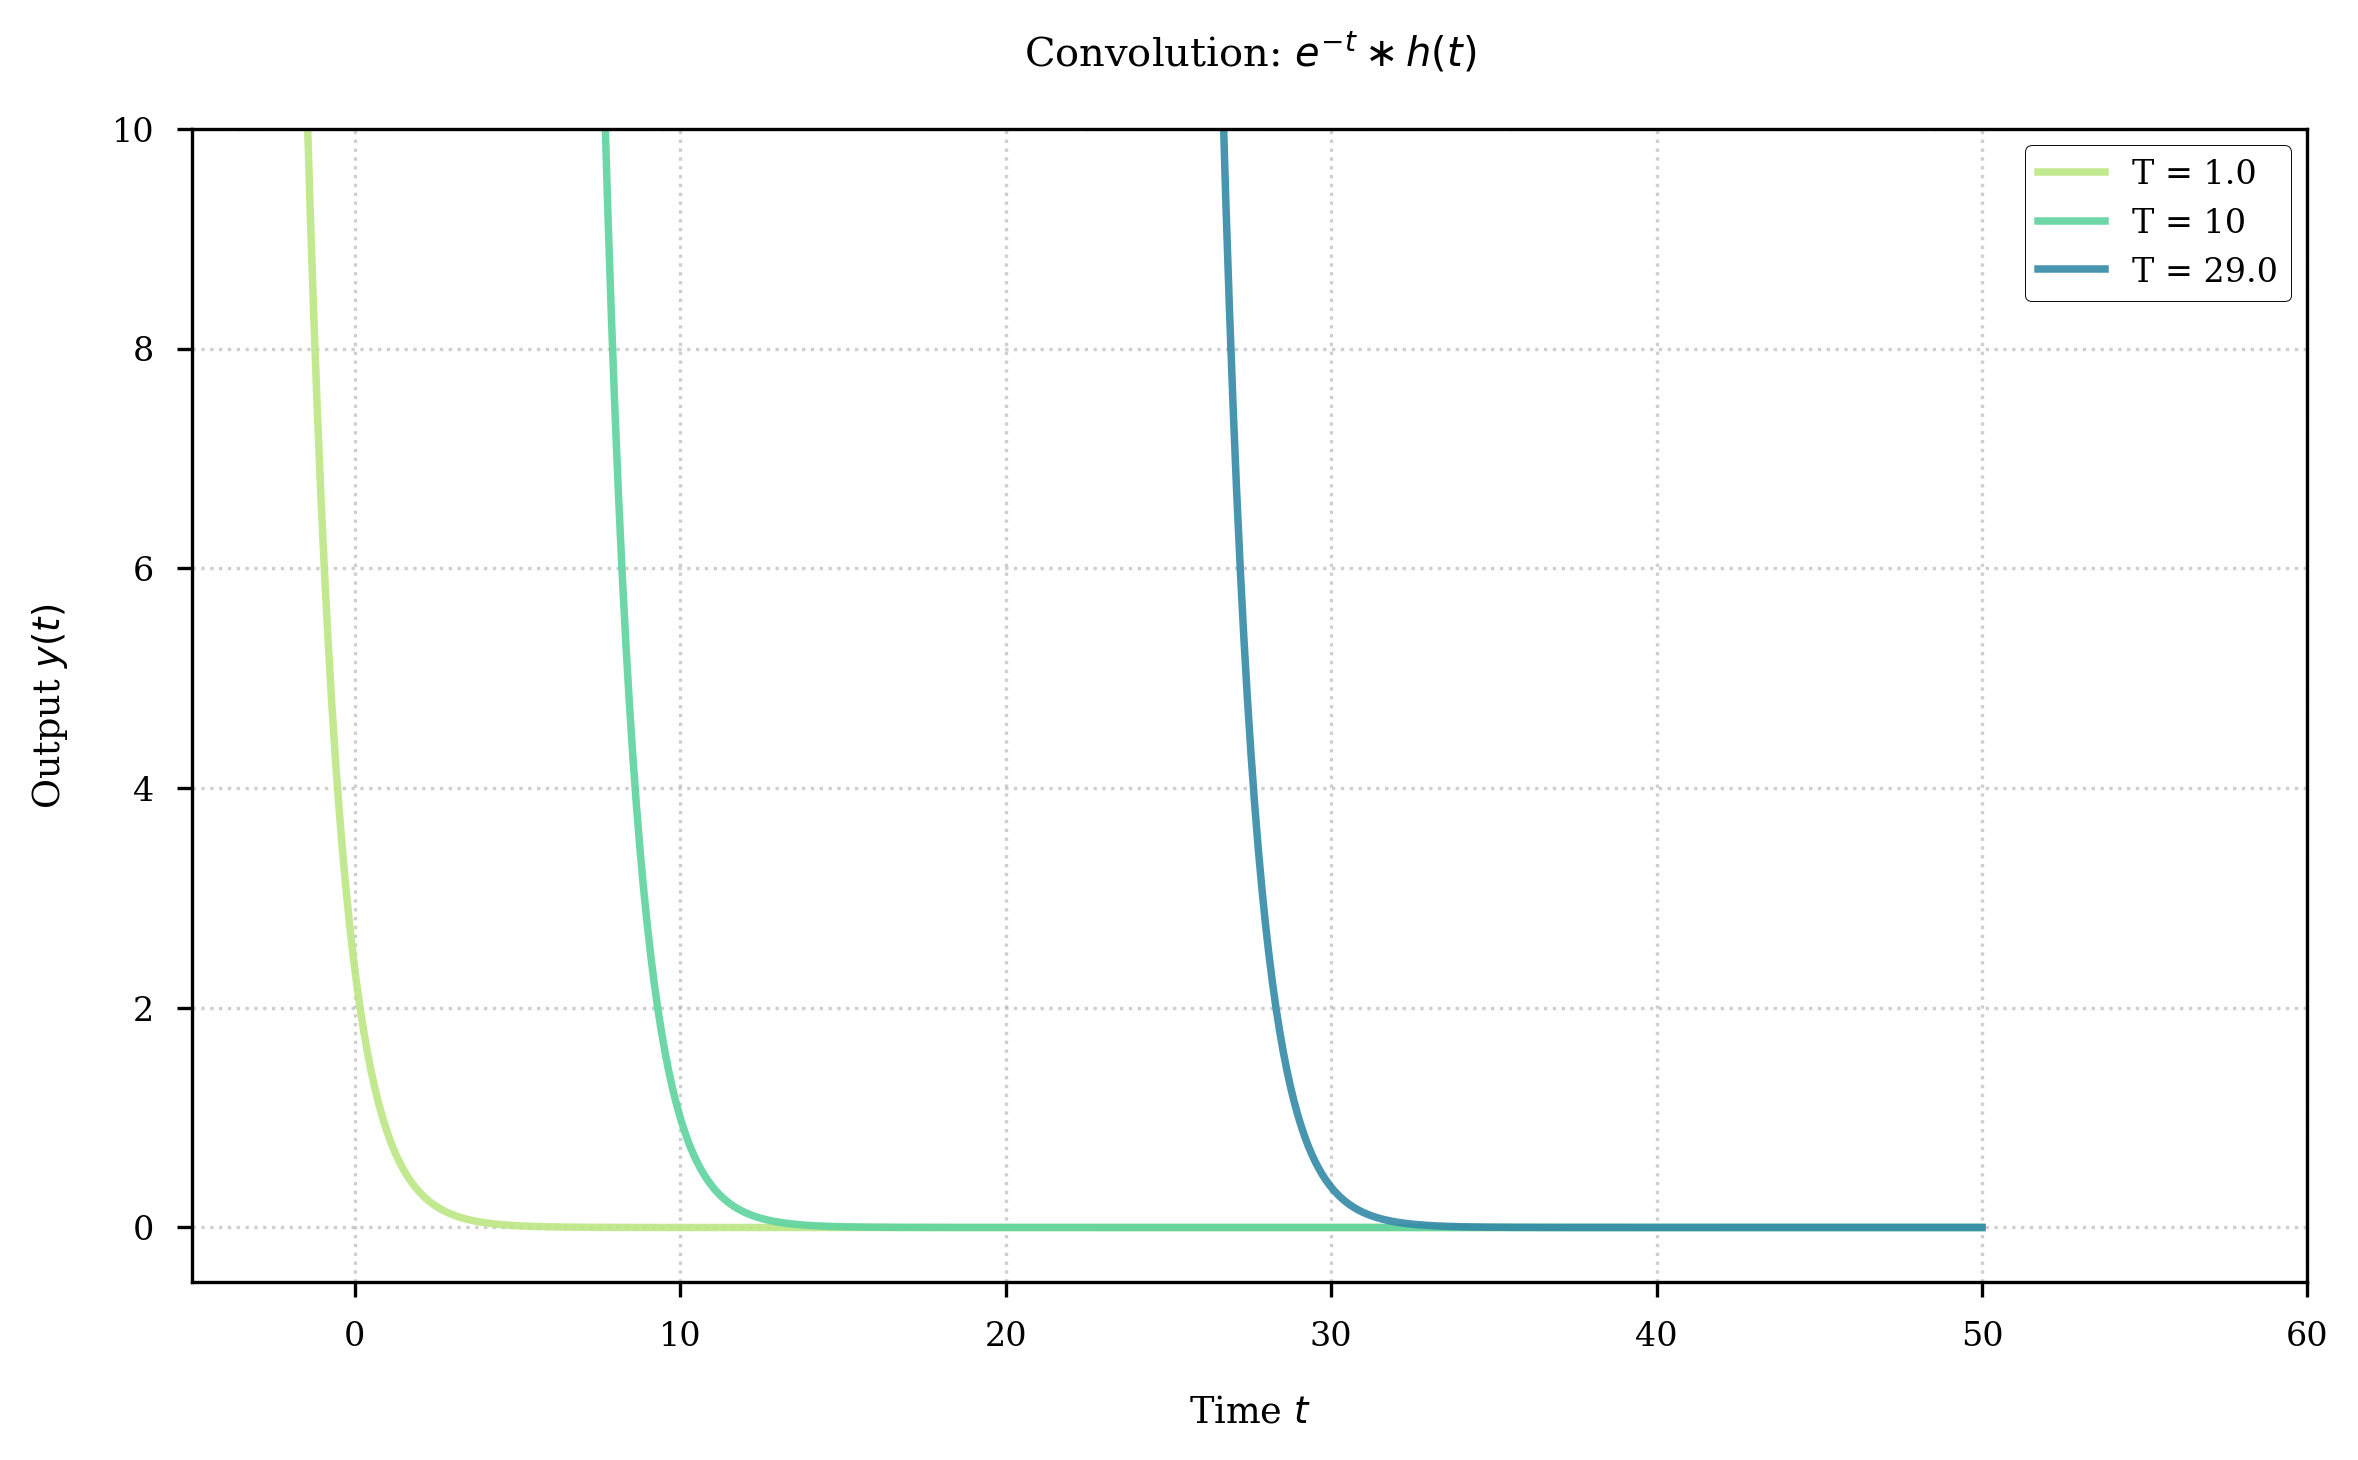
\includegraphics[width=0.8\textwidth]{figs/exp_convolution.png}
		\caption{Convolution of $f(t) = e^{-t}$ with a rectangular kernel for varying values of $T$. As $T$ increases, the output signal amplitude scales by $\frac{2\sinh(aT)}{a}$ but retains the exponential decay nature. For large values of $T$ (e.g., $T = 29.0$), the output achieves relatively higher amplitudes (approximately 8) than smaller $T$ values, showing the amplification property of the width of the rectangular kernel without losing the exponential nature of the original function.}
		\label{fig:exp_convolution}
	\end{figure}
	
	\section{Convolution with Hyperbolic Function}
	Let's consider $f(t) = \sinh(bt)$ for $b > 0$.
	
	The convolution is:
	\begin{equation}
		y(t) = \int_{-\infty}^{\infty} \sinh(b\tau) \cdot h(t - \tau) d\tau = \int_{t-T}^{t+T} \sinh(b\tau) d\tau
	\end{equation}
	
	Computing this integral:
	\begin{align}
		y(t) &= \int_{t-T}^{t+T} \sinh(b\tau) d\tau \\
		&= \left[ \frac{1}{b}\cosh(b\tau) \right]_{t-T}^{t+T} \\
		&= \frac{1}{b}(\cosh(b(t+T)) - \cosh(b(t-T)))
	\end{align}
	
	Using the identity $\cosh(A) - \cosh(B) = 2\sinh(\frac{A+B}{2})\sinh(\frac{A-B}{2})$:
	\begin{align}
		y(t) &= \frac{1}{b}(2\sinh(bt)\sinh(bT)) \\
		&= \frac{2\sinh(bT)}{b}\sinh(bt)
	\end{align}
	
	\begin{figure}[htbp]
		\centering
		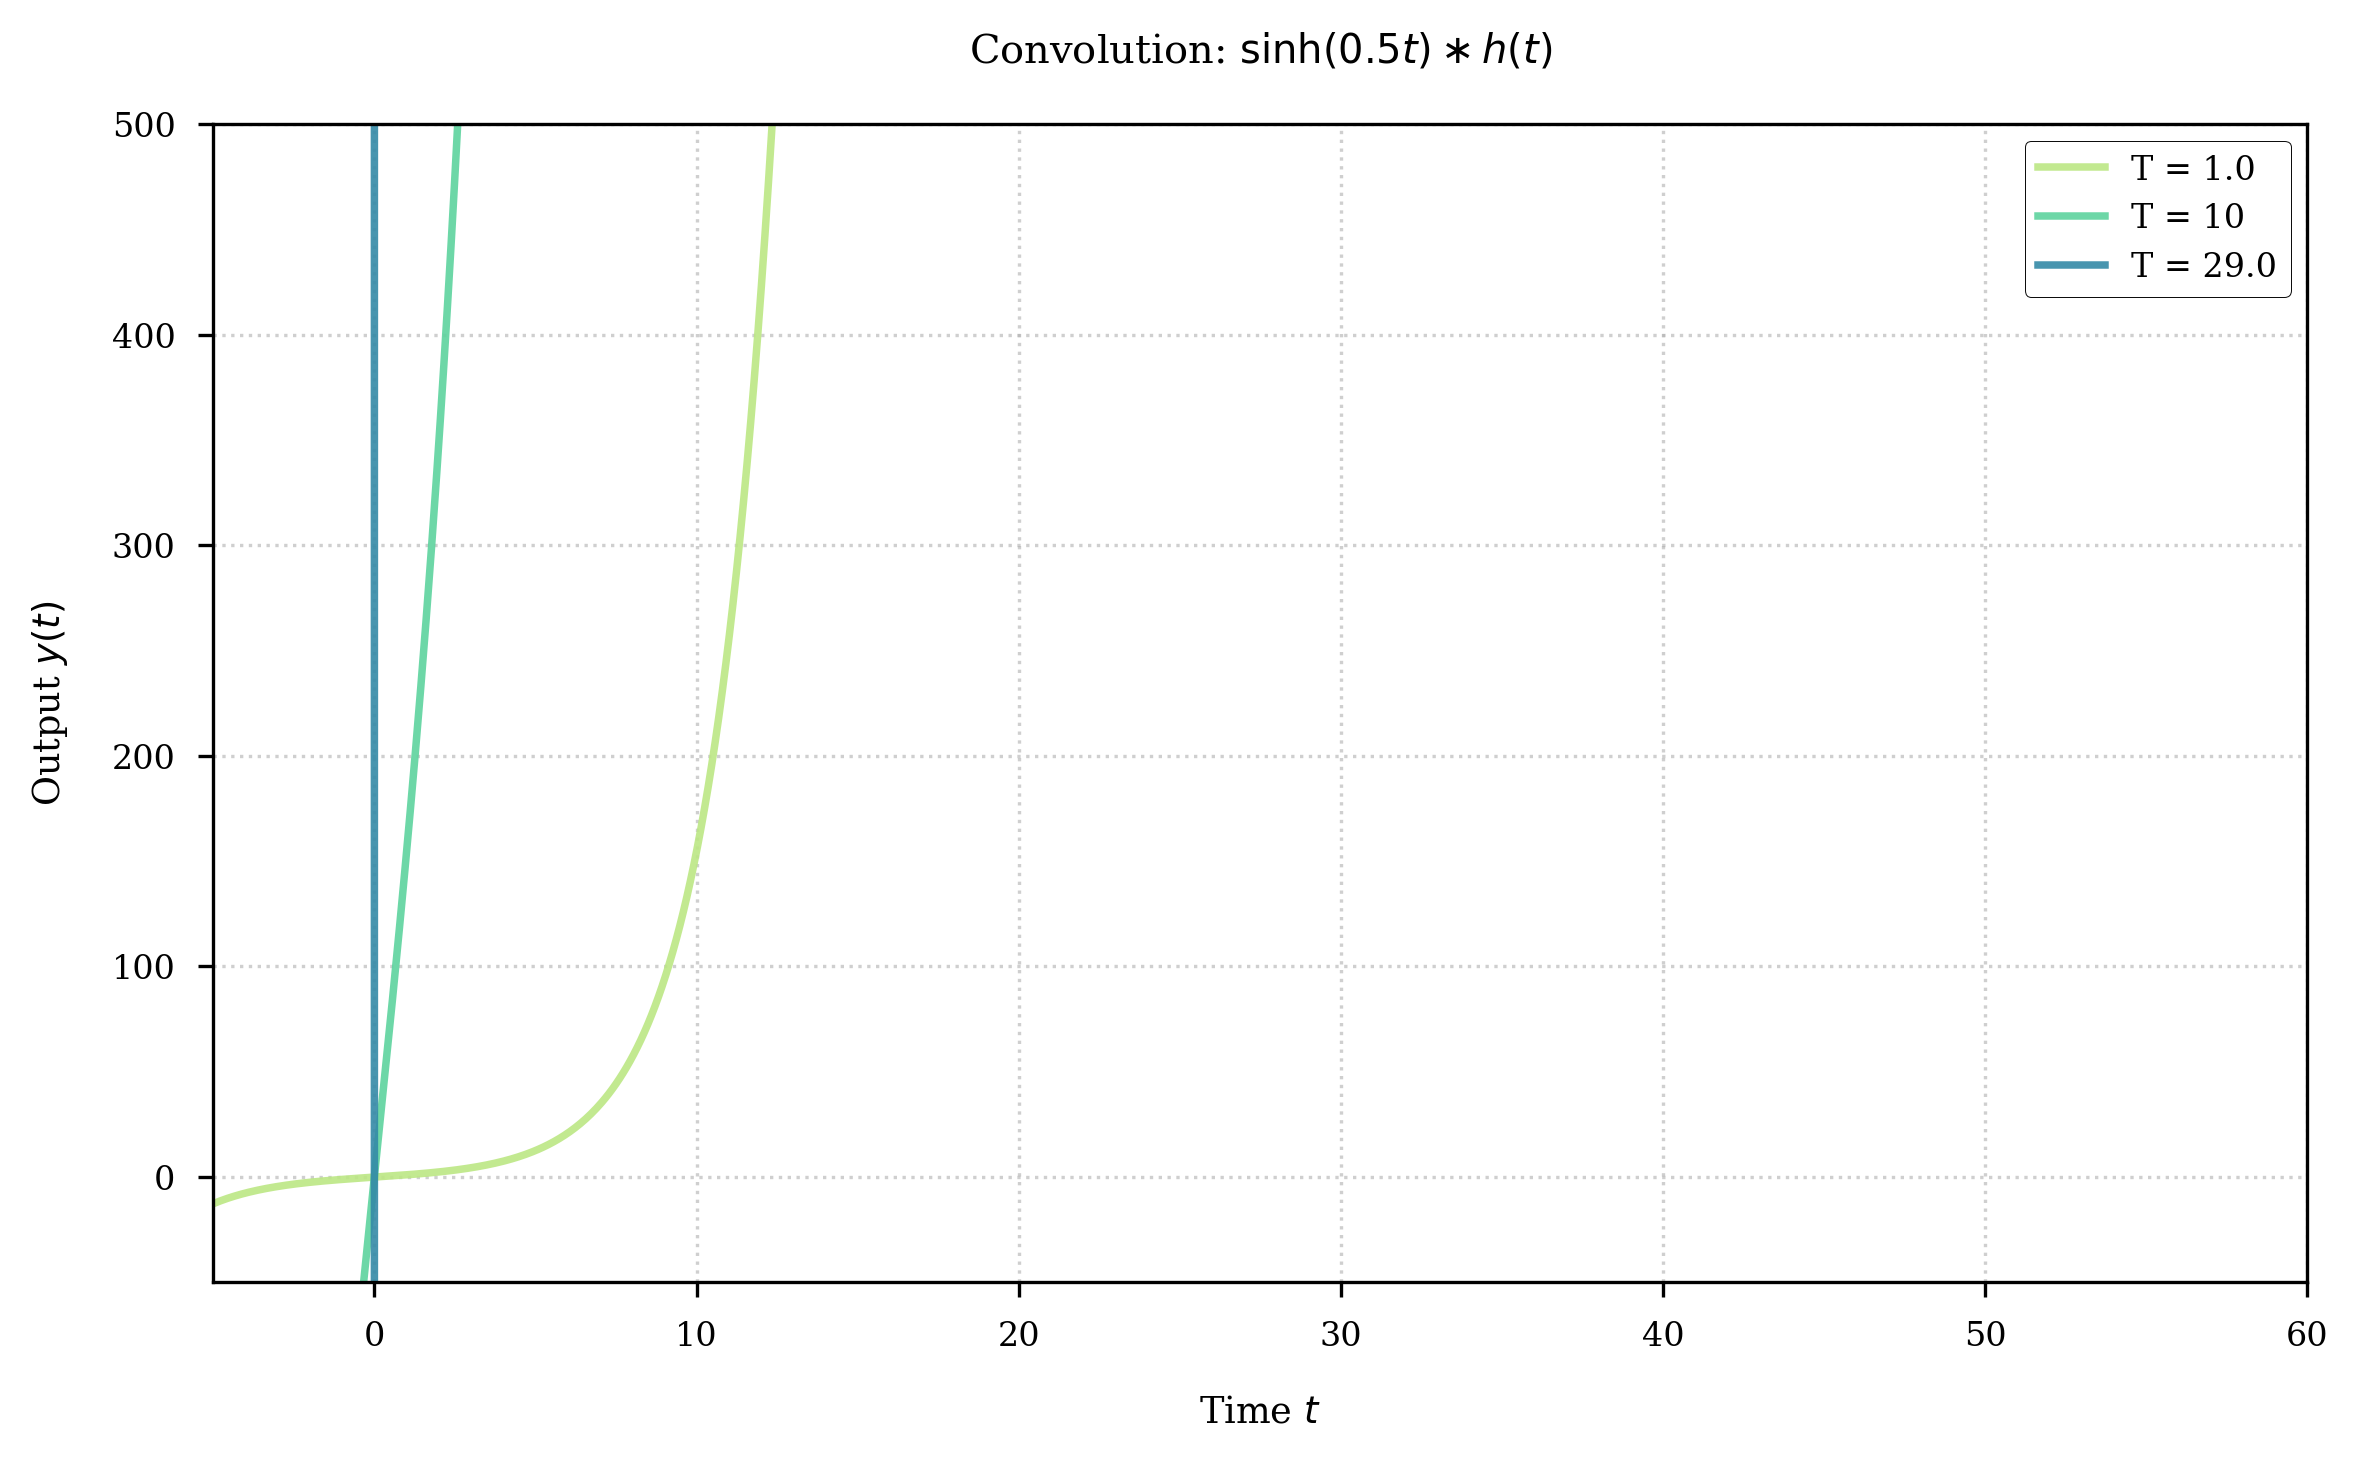
\includegraphics[width=0.8\textwidth]{figs/hyper_convolution.png}
		\caption{Convolution of $f(t) = \sinh(0.5t)$ with a rectangular kernel of varying $T$. The output retains the hyperbolic sine form but with increased magnitude that varies with $\frac{2\sinh(bT)}{b}$. With an increase in $T$, the amplitude increases significantly, reaching around $\pm100$ for $T = 29.0$. In contrast to the exponential scenario, this output increases both positively and negatively, illustrating the way the wider rectangular kernels increase the hyperbolic nature of the original function.}
		\label{fig:hyper_convolution}
	\end{figure}
	
	\subsection{Modified Kernel Analysis}
	\subsubsection{Kernel for $t > 0$ (Part a)}
	For part (a), we need to modify the kernel to only consider the part for $t > 0$:
	\begin{equation}
		h_m(t) = 
		\begin{cases} 
			1, & \text{for } 0 \leq t \leq T \\
			0, & \text{otherwise}
		\end{cases}
	\end{equation}
	
	This is equivalent to applying a unit step function to the original kernel and adjusting the range:
	\begin{equation}
		h_m(t) = h(t+T) \cdot u(t)
	\end{equation}
	
	For the exponential function $f(t) = e^{-at}$, we now need to introduce the step function $u(t)$ for a causal system analysis. Let's define $f_c(t) = e^{-at}u(t)$ for $a > 0$.
	
	The convolution becomes:
	\begin{equation}
		y_m(t) = \int_{-\infty}^{\infty} e^{-a\tau}u(\tau) \cdot h_m(t - \tau) d\tau
	\end{equation}
	
	The effective integration limits are determined by where both $\tau \geq 0$ and $0 \leq t - \tau \leq T$, or $t - T \leq \tau \leq t$ and $\tau \geq 0$:
	\begin{equation}
		y_m(t) = \int_{\max(0, t-T)}^{\min(t, t)} e^{-a\tau} d\tau
	\end{equation}
	
	Analyzing different cases:
	
	\subsubsection{Case 1: $t < 0$}
	In this case, $\min(t, t) = t < 0$, so there's no overlap and $y_m(t) = 0$.
	
	\subsubsection{Case 2: $0 \leq t < T$}
	Here, $t - T < 0$ and $t \geq 0$, so:
	\begin{align}
		y_m(t) &= \int_{0}^{t} e^{-a\tau} d\tau \\
		&= \frac{1}{a}(1 - e^{-at})
	\end{align}
	
	\subsubsection{Case 3: $t \geq T$}
	Both $t - T \geq 0$ and $t > 0$, so:
	\begin{align}
		y_m(t) &= \int_{t-T}^{t} e^{-a\tau} d\tau \\
		&= \frac{1}{a}(e^{-a(t-T)} - e^{-at}) \\
		&= \frac{e^{-at}}{a}(e^{aT} - 1)
	\end{align}
	
	Therefore, the complete convolution result for the modified kernel is:
	\begin{equation}
		y_m(t) = 
		\begin{cases} 
			0, & t < 0 \\
			\frac{1}{a}(1 - e^{-at}), & 0 \leq t < T \\
			\frac{e^{-at}}{a}(e^{aT} - 1), & t \geq T
		\end{cases}
	\end{equation}
	
	\begin{figure}[htbp]
		\centering
		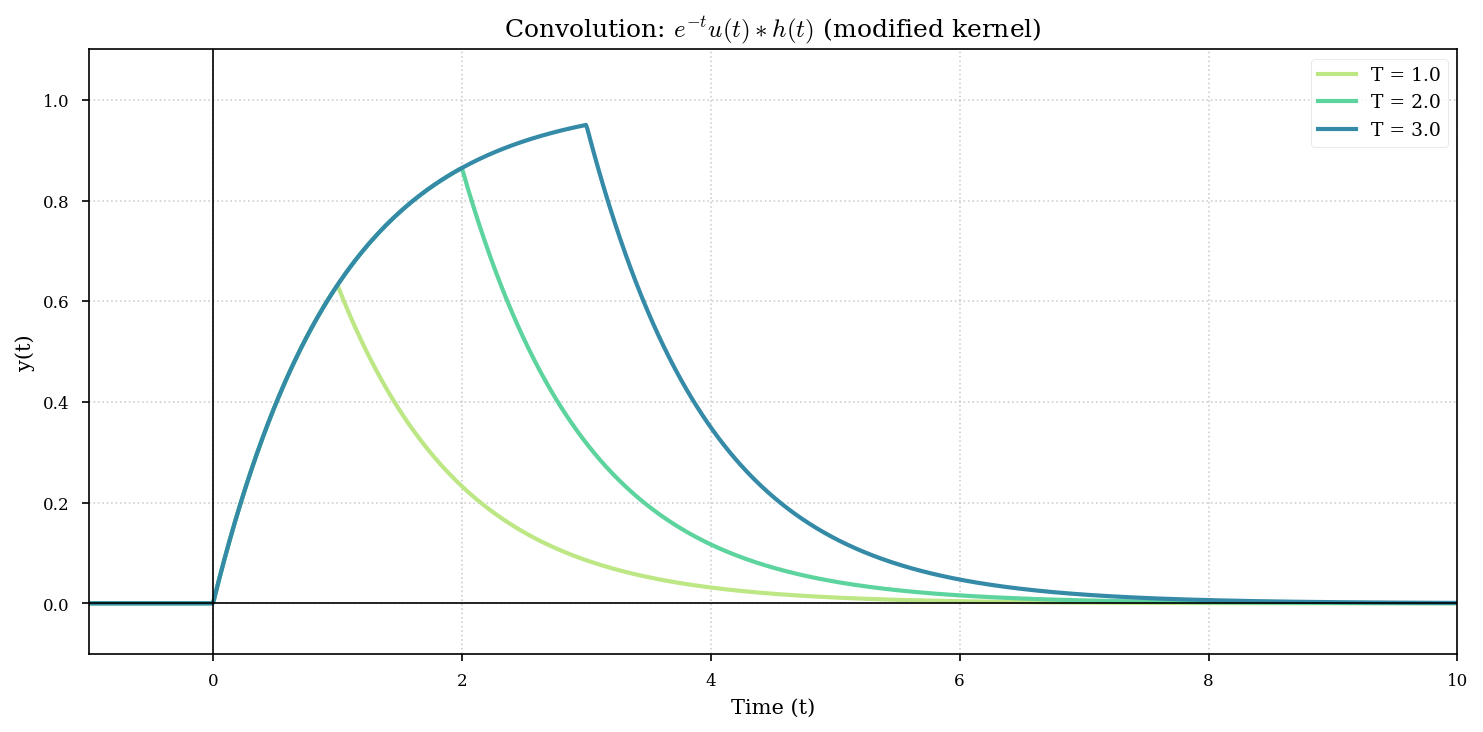
\includegraphics[width=0.8\textwidth]{figs/exp_modified_convolution.png}
		\caption{Convolution of $f(t) = e^{-t}u(t)$ with the modified kernel for various values of $T$. The result is zero for $t < 0$ due to causality. For $0 \leq t < T$, the response rises as $(1 - e^{-at})/a$ to various maximum levels depending on $T$. For $t \geq T$, the output takes an exponential decay form $e^{-at}(e^{aT} - 1)/a$. Higher values of $T$ produce greater peak amplitudes and broader response regions. For $T = 3.0$, the peak is about 0.95 at $t \approx 3$, with exponential decay thereafter.}
		\label{fig:exp_modified_convolution}
	\end{figure}
	
	\subsection{Hyperbolic Function with Modified Kernel}
	For the hyperbolic function with the modified kernel, a similar analysis gives:
	
	\subsubsection{Case 1: $t < 0$}
	The output is zero: $y_m(t) = 0$.
	
	\subsubsection{Case 2: $0 \leq t < T$}
	\begin{align}
		y_m(t) &= \int_{0}^{t} \sinh(b\tau) d\tau \\
		&= \frac{1}{b}(\cosh(bt) - 1)
	\end{align}
	
	\subsubsection{Case 3: $t \geq T$}
	\begin{align}
		y_m(t) &= \int_{t-T}^{t} \sinh(b\tau) d\tau \\
		&= \frac{1}{b}(\cosh(bt) - \cosh(b(t-T)))
	\end{align}
	
	Using the identity $\cosh(A) - \cosh(B) = 2\sinh(\frac{A+B}{2})\sinh(\frac{A-B}{2})$:
	\begin{align}
		y_m(t) &= \frac{1}{b}(2\sinh(b(t-\frac{T}{2}))\sinh(\frac{bT}{2})) \\
		&= \frac{2\sinh(\frac{bT}{2})}{b}\sinh(b(t-\frac{T}{2}))
	\end{align}
	
	Therefore, the complete convolution result is:
	\begin{equation}
		y_m(t) = 
		\begin{cases} 
			0, & t < 0 \\
			\frac{1}{b}(\cosh(bt) - 1), & 0 \leq t < T \\
			\frac{2\sinh(\frac{bT}{2})}{b}\sinh(b(t-\frac{T}{2})), & t \geq T
		\end{cases}
	\end{equation}
	
	\begin{figure}[htbp]
		\centering
		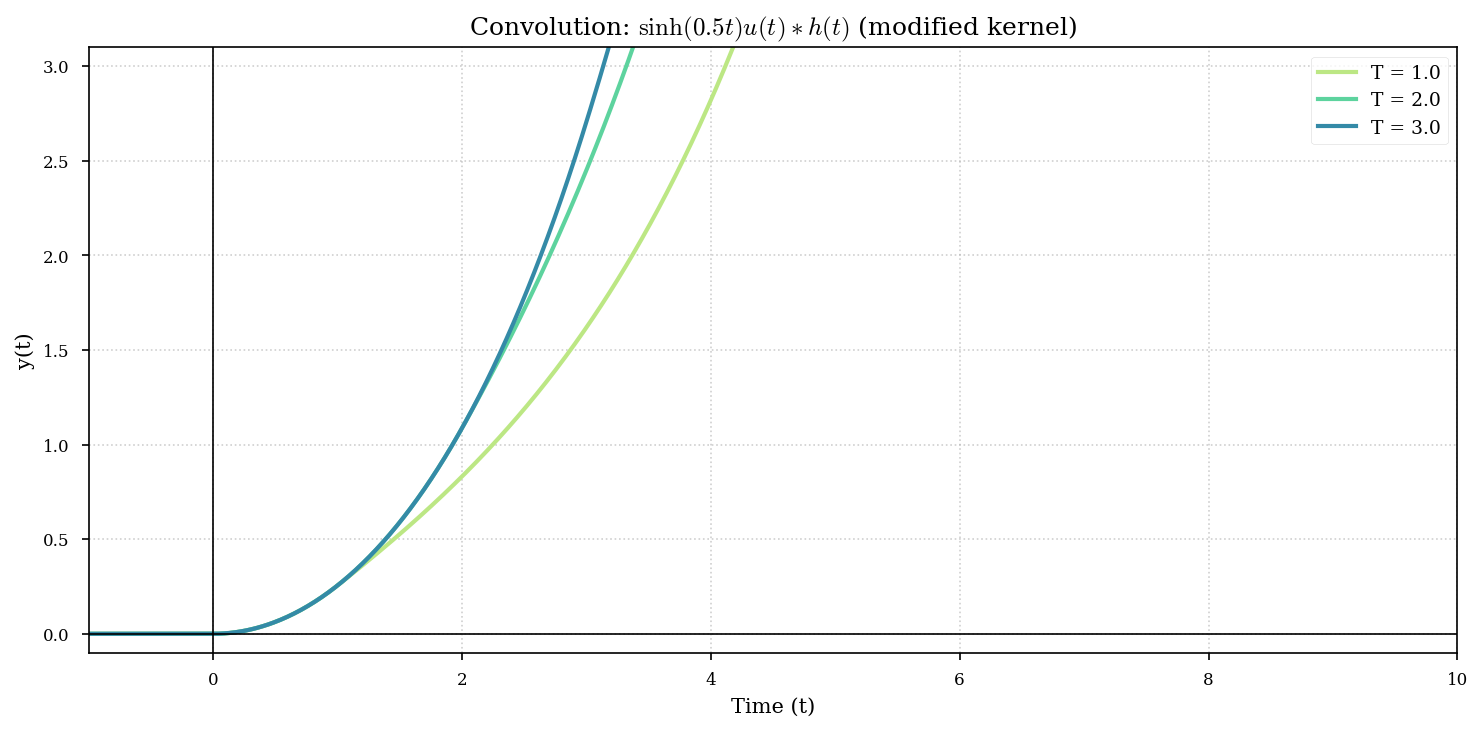
\includegraphics[width=0.8\textwidth]{figs/hyper_modified_convolution.png}
		\caption{Convolution of $f(t) = \sinh(0.5t)u(t)$ with the modified kernel for various values of $T$. The result is zero for $t < 0$, and for $t > 0$ has exponential growth properties of the hyperbolic sine function. As $T$ grows, the rate of growth becomes faster, with the $T = 3.0$ curve having the most rapid growth. In contrast to the exponential case, these curves still rise without limit after $t = T$, with the pattern $\frac{2\\sinh(\frac{bT}{2})}{b}\sinh(b(t-\frac{T}{2}))$. All three curves approach each other for small $t$ but spread out considerably as $t$ grows, illustrating how the system exaggerates the input signal more with wider kernels.}
		\label{fig:hyper_modified_convolution}
	\end{figure}
	
	\subsection{Time-Shifted Kernel (Part b)}
	For part (b), we analyze a kernel shifted by a time $\tau_0$:
	\begin{equation}
		h_s(t) = 
		\begin{cases} 
			1, & \text{for } -T+\tau_0 \leq t \leq T+\tau_0 \\
			0, & \text{otherwise}
		\end{cases}
	\end{equation}
	
	This is equivalent to:
	\begin{equation}
		h_s(t) = h(t-\tau_0)
	\end{equation}
	
	\subsubsection{Exponential Function with Time-Shifted Kernel}
	The convolution with $f(t) = e^{-at}$ becomes:
	\begin{equation}
		y_s(t) = \int_{-\infty}^{\infty} e^{-a\tau} \cdot h_s(t - \tau) d\tau = \int_{-\infty}^{\infty} e^{-a\tau} \cdot h(t - \tau - \tau_0) d\tau
	\end{equation}
	
	Using the time-shifting property of convolution, we can write:
	\begin{equation}
		y_s(t) = y(t-\tau_0) = \frac{2\sinh(aT)}{a}e^{-a(t-\tau_0)} = \frac{2\sinh(aT)}{a}e^{a\tau_0}e^{-at}
	\end{equation}
	
	This shows that shifting the kernel by $\tau_0$ results in a time-shift of the output and an amplitude scaling by $e^{a\tau_0}$.
	
	\begin{figure}[htbp]
		\centering
		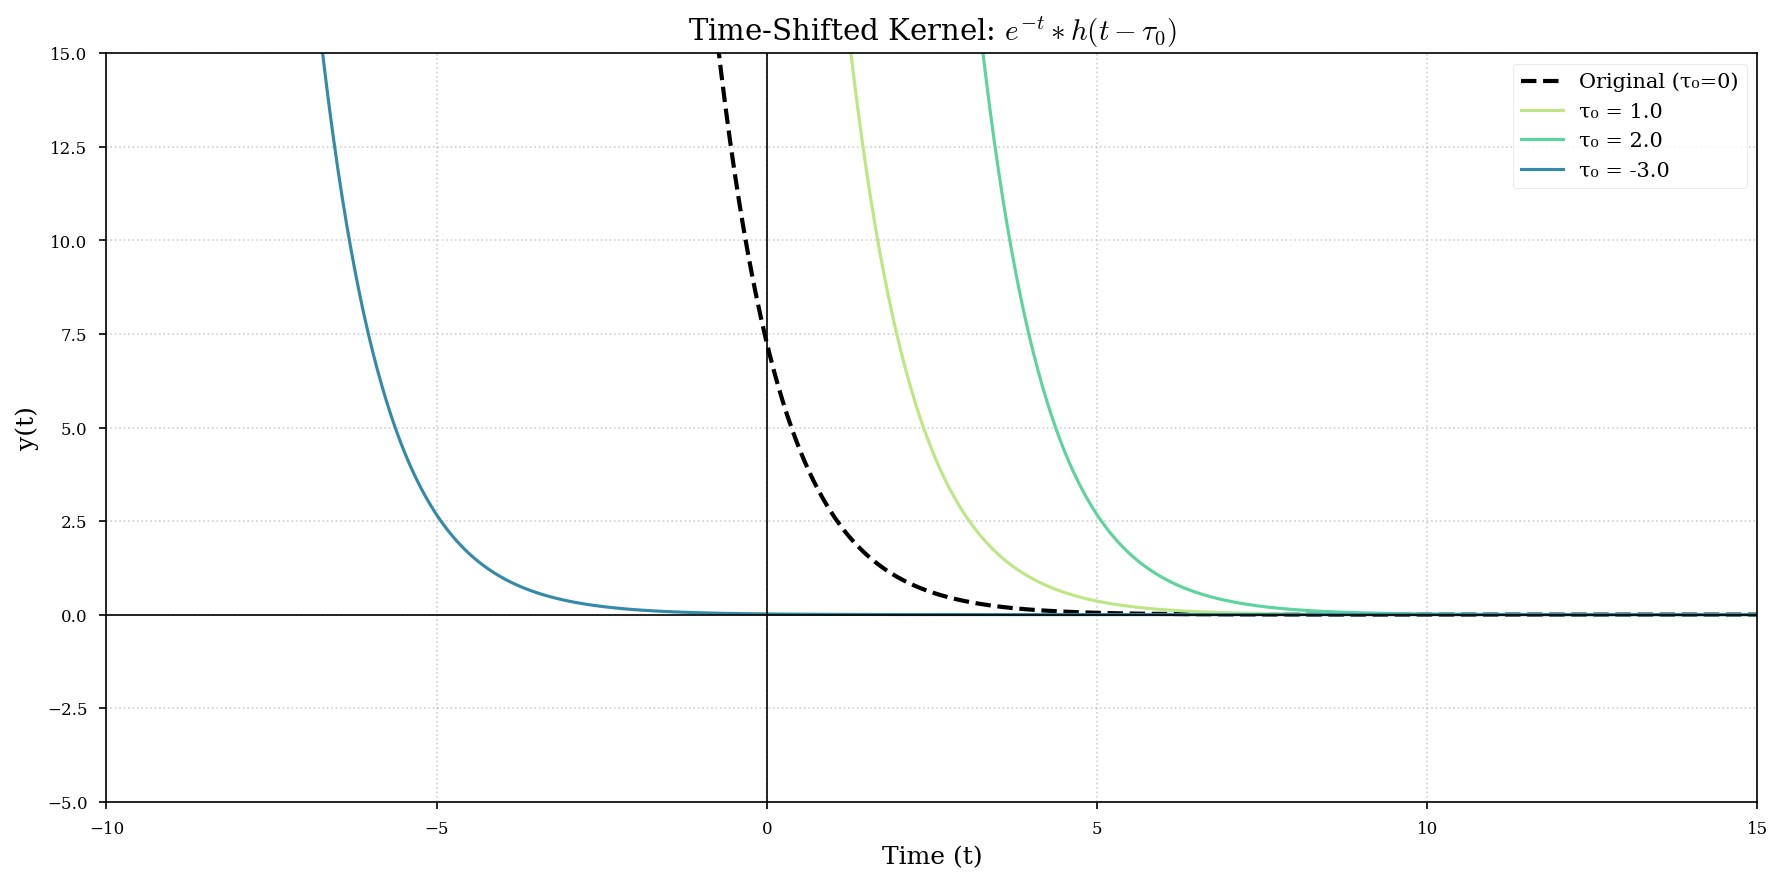
\includegraphics[width=0.8\textwidth]{figs/exp_time_shift_extended.png}
		\caption{Convolution of $f(t) = e^{-t}$ with time-shifted rectangular kernel $h(t-\tau_0)$ for various values of $\tau_0$. The original response ($\tau_0 = 0$) is represented as a dashed line. As $\tau_0$ is increased, the whole response curve is shifted to the right by $\tau_0$ and scaled by a factor of $e^{\tau_0}$. For $\tau_0 = 1.0$, the curve is shifted right by 1 unit and scales up in amplitude. For $\tau_0 = 2.0$, the shift is 2 units with additional amplification. Similarly, for $\tau_0 = -3.0$, the shift is 3 units to the left. All curves share the typical exponential decay but different initial points and amplitudes, according to the equation $\frac{2\sinh(aT)}{a}e^{a\tau_0}e^{-at}$.}
		\label{fig:exp_shifted_kernel}
	\end{figure}
	
	\subsubsection{Hyperbolic Function with Time-Shifted Kernel}
	For the hyperbolic function $f(t) = \sinh(bt)$, the convolution with the time-shifted kernel is:
	\begin{equation}
		y_s(t) = \int_{-\infty}^{\infty} \sinh(b\tau) \cdot h_s(t - \tau) d\tau = \int_{-\infty}^{\infty} \sinh(b\tau) \cdot h(t - \tau - \tau_0) d\tau
	\end{equation}
	
	Using the time-shifting property of convolution, the result is:
	\begin{equation}
		y_s(t) = y(t-\tau_0) = \frac{2\sinh(bT)}{b}\sinh(b(t-\tau_0))
	\end{equation}
	
	This represents a pure time-shift of the original response without amplitude scaling, unlike the exponential case.
	
	\begin{figure}[htbp]
		\centering
		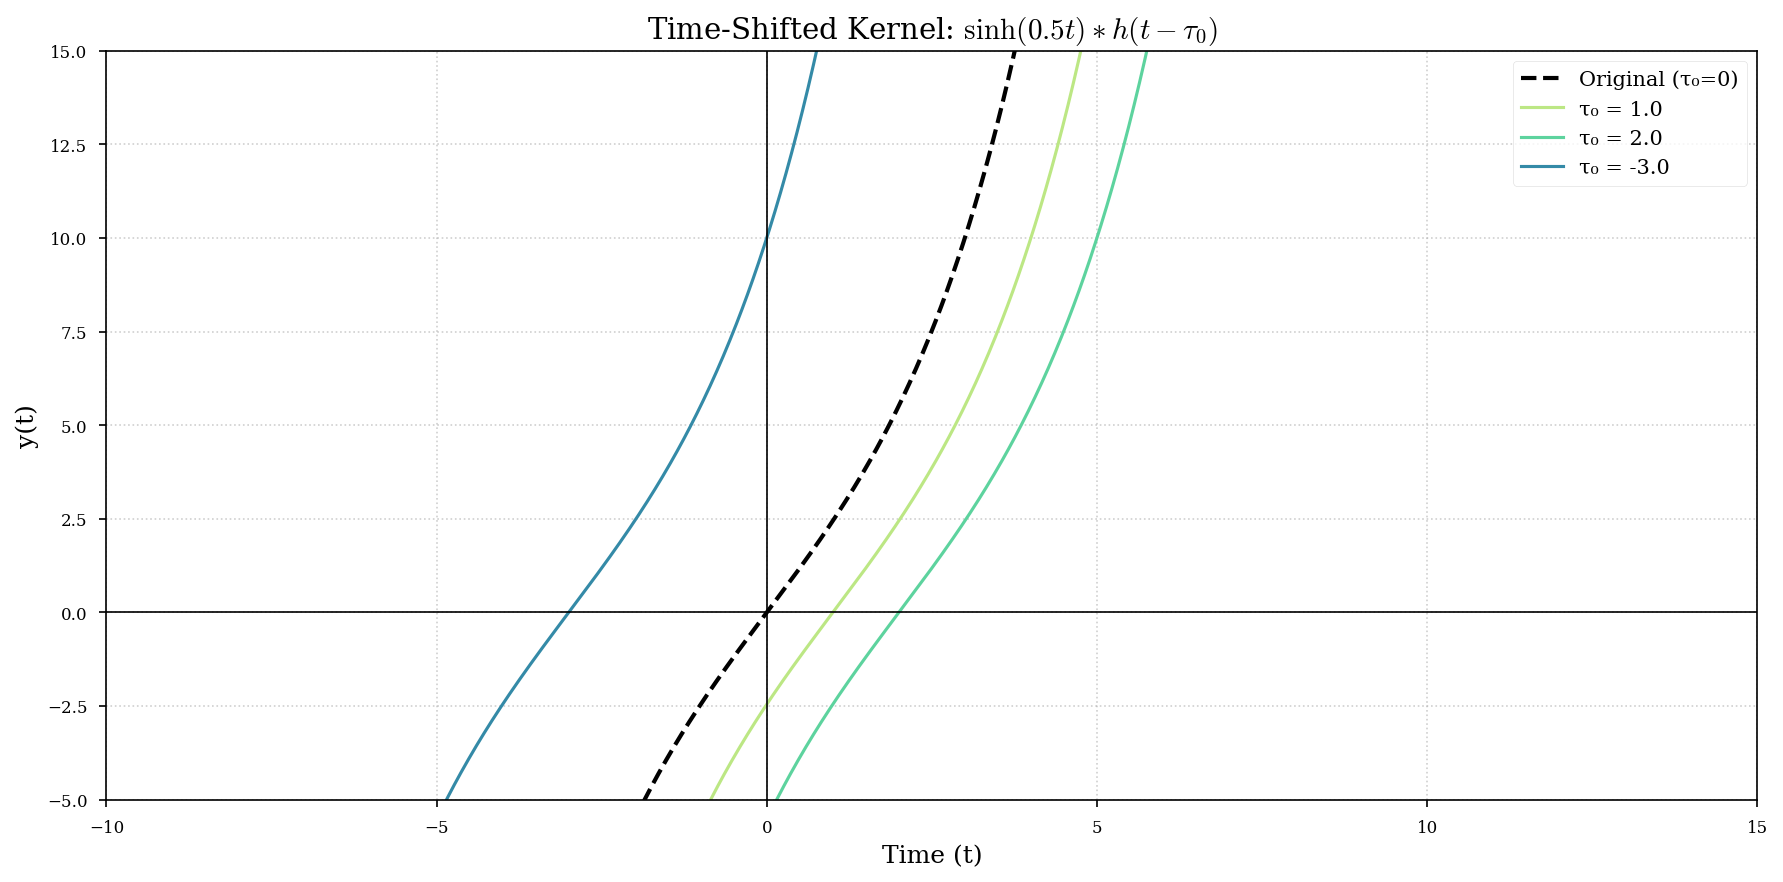
\includegraphics[width=0.8\textwidth]{figs/hyper_time_shift_extended.png}
		\caption{Convolution of $f(t) = \sinh(0.5t)$ with time-shifted rectangular kernel $h(t-\tau_0)$ for various values of $\tau_0$. The original response ($\tau_0 = 0$) is a dashed line. For increasing values of $\tau_0$, the response curves move horizontally to the right by $\tau_0$ units. For $\tau_0 = 1.0$, the curve moves right by 1 unit, for $\tau_0 = 2.0$, the move is 2 units and for $\tau_0 = -3.0$, its 3 units to the left. In contrast to the exponential case, there is no scaling of amplitude - just a simple time-shift, as seen in the parallel curves. Every curve is described by the equation $\frac{2\sinh(bT)}{b}\sinh(b(t-\tau_0))$, with the same hyperbolic growth rate but with varying x-intercepts at $t = \tau_0$.}
	\end{figure}
	
	\subsection{Comparison of Exponential and Hyperbolic Functions with Time-Shifted Kernels}
	The time-shifted kernel brings out the key distinction between exponential and hyperbolic functions in convolution systems:
	
	
	\begin{itemize}
		\item For the exponential function $f(t) = e^{-at}$, a time-shift in the kernel results in both a time-shift and amplitude scaling in the output. The scaling factor $e^{a\\tau_0}$ grows exponentially with the amount of the shift.
		\item For the hyperbolic function $f(t) = \sinh(bt)$, a time-shift in the kernel results only in a time-shift in the output and not in amplitude scaling. The curves do not change their shape and are merely shifted horizontally.
	\end{itemize}

